\section{Experiment Analysis}
In this part, we will implement several unconstrained and constrained optimization alogorithms to solve minimum surfaces and obstacle problems respectively. More specificly, we will employ 3 basic unconstrained optimization algorithms (gradient descent method with backtracking, globalized Newton method, L- BFGS method) with 5 different boundary functions in the minimum surface problems. We will also consider how the discretization degree and addtional techniques influence our experimental results. For the obstacle problem, we will apply two constrained optimization algorithms (quadratic penalty method and projected gradient method) in combination with different obstacle functions. And meanwhile, we will analyze the perfomance of different implemented algorithms and discuss some potential improvements.
\subsection{Minimum Surfaces}
At first, we will illustrate five different boundary functions. Then we will choose one advanced algorithm to solve the minimum surface problem with five boundary functions and different discretization degree. Subsequently, we utilize other unconstrained optimization alogorithms and compare their perfomance from the perspective of relative objective function gap and iteration of norm of gradients. Finally, additional techniques such as exact line search, Barzilai-Borwein steps and inertial techniques will be introduced to accelerate the convergence process.
\subsubsection{Boundary Functions}
Here, figure \ref{fig:boundary} presents five different boundary function mentioned in the report requirement document. We will then determine the minimum surfaces using different boundary functions via our proposed algorithms.
\begin{figure}[!htbp]
    \centering
    \subfigure[$ r_1(x, y)=1+\sin (2 \pi x)$]
    {
    \centering
    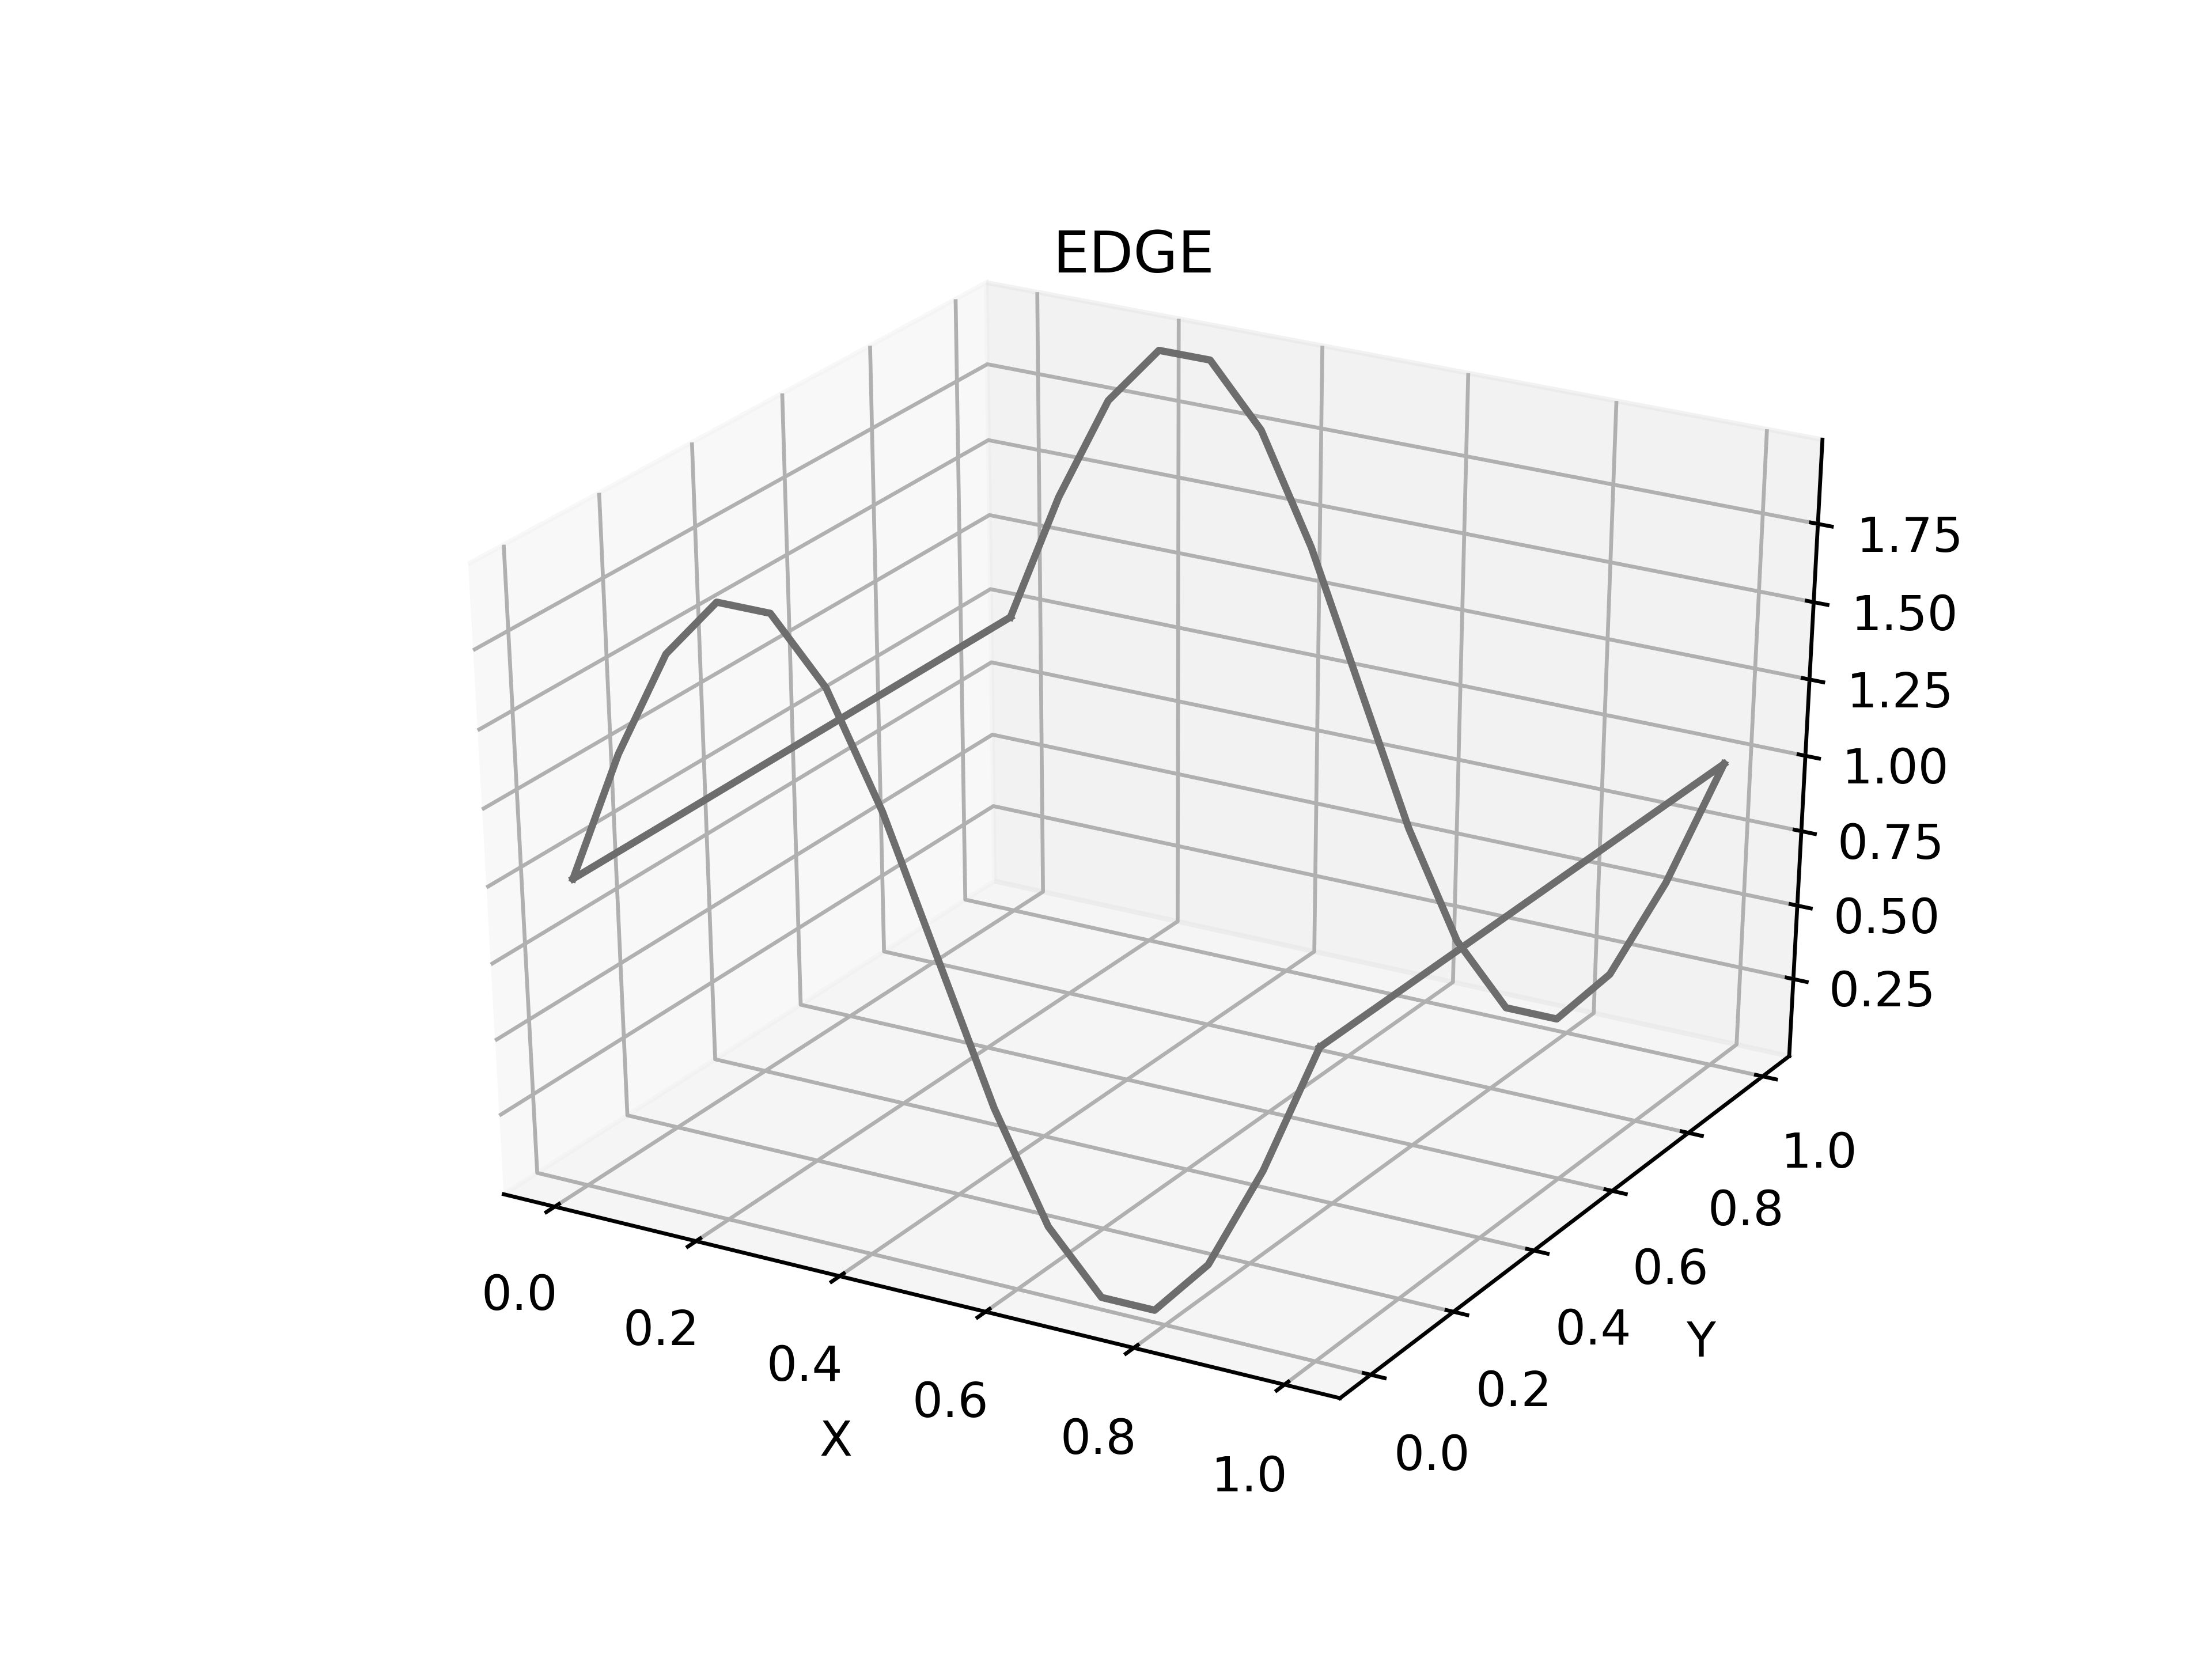
\includegraphics[width=0.3\columnwidth]{images/boundary_1.png}
    }
    \subfigure[$ r_2(x, y)=1+\cos (1 / (x+0.001) )$]
    {
    \centering
    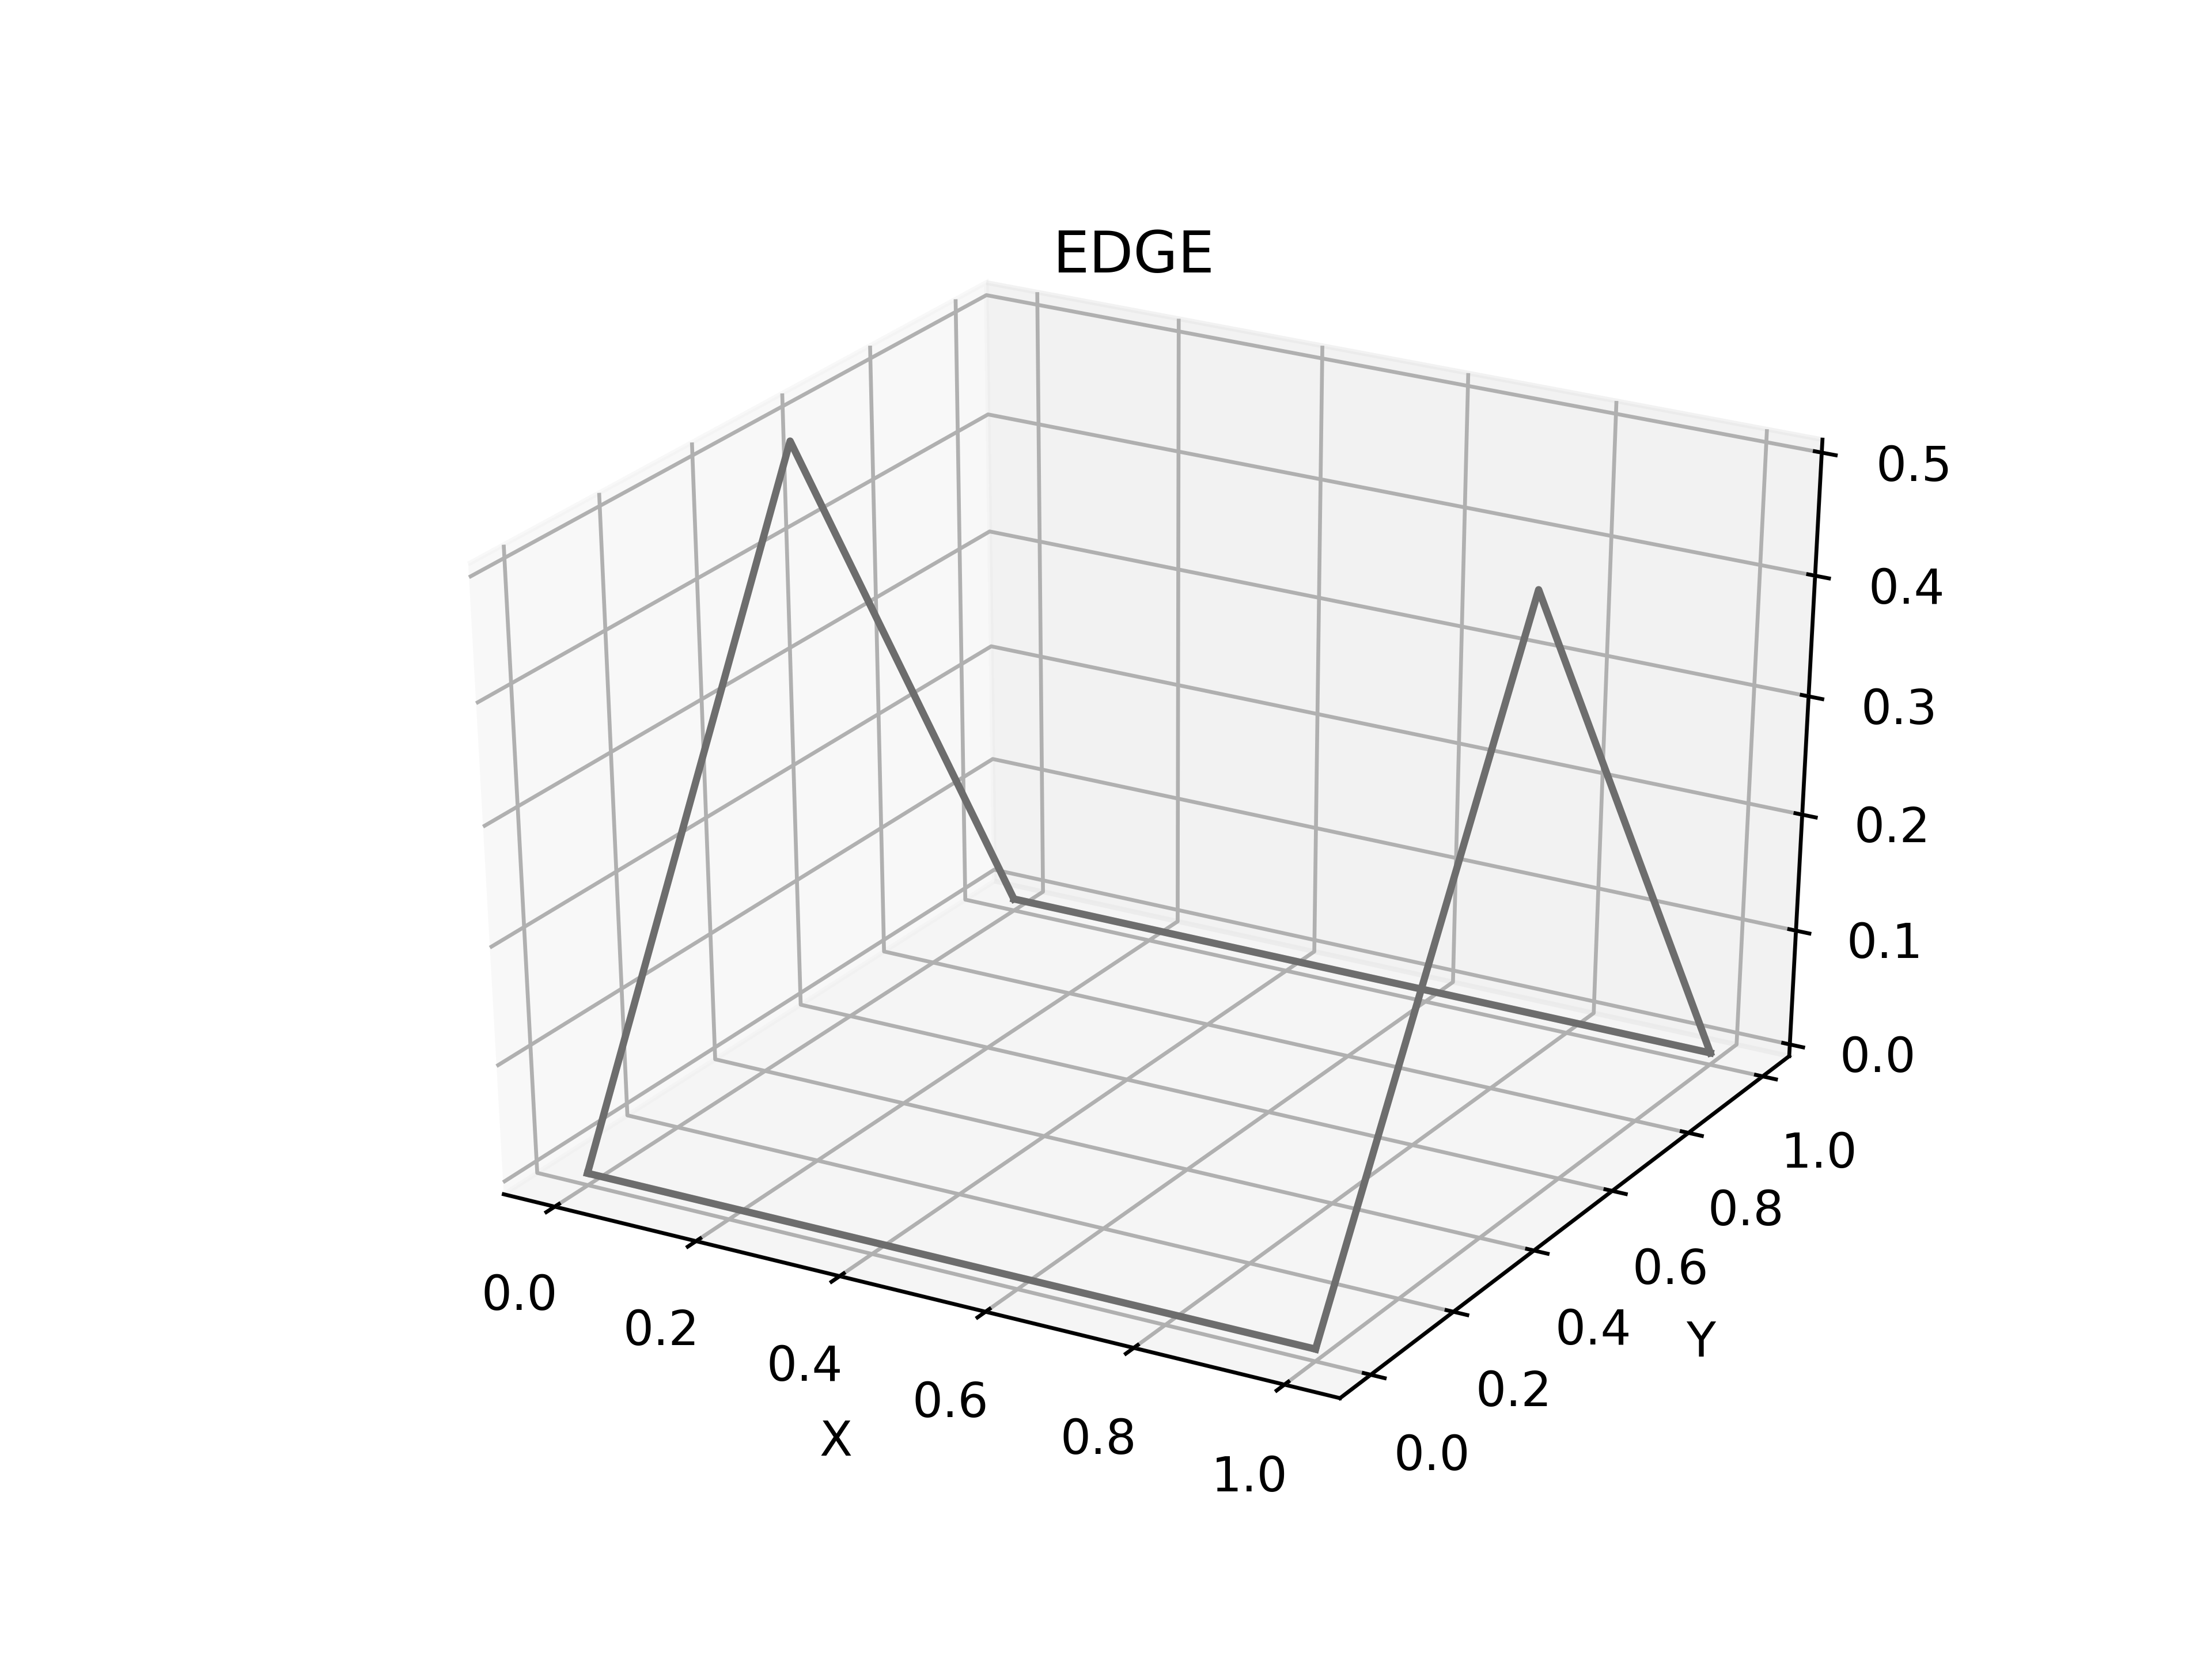
\includegraphics[width=0.3\columnwidth]{images/boundary_2.png}
    }
    \subfigure[$ r_3(x, y)=\frac{1}{2}-\left|y-\frac{1}{2}\right|$]
    {
    \centering
    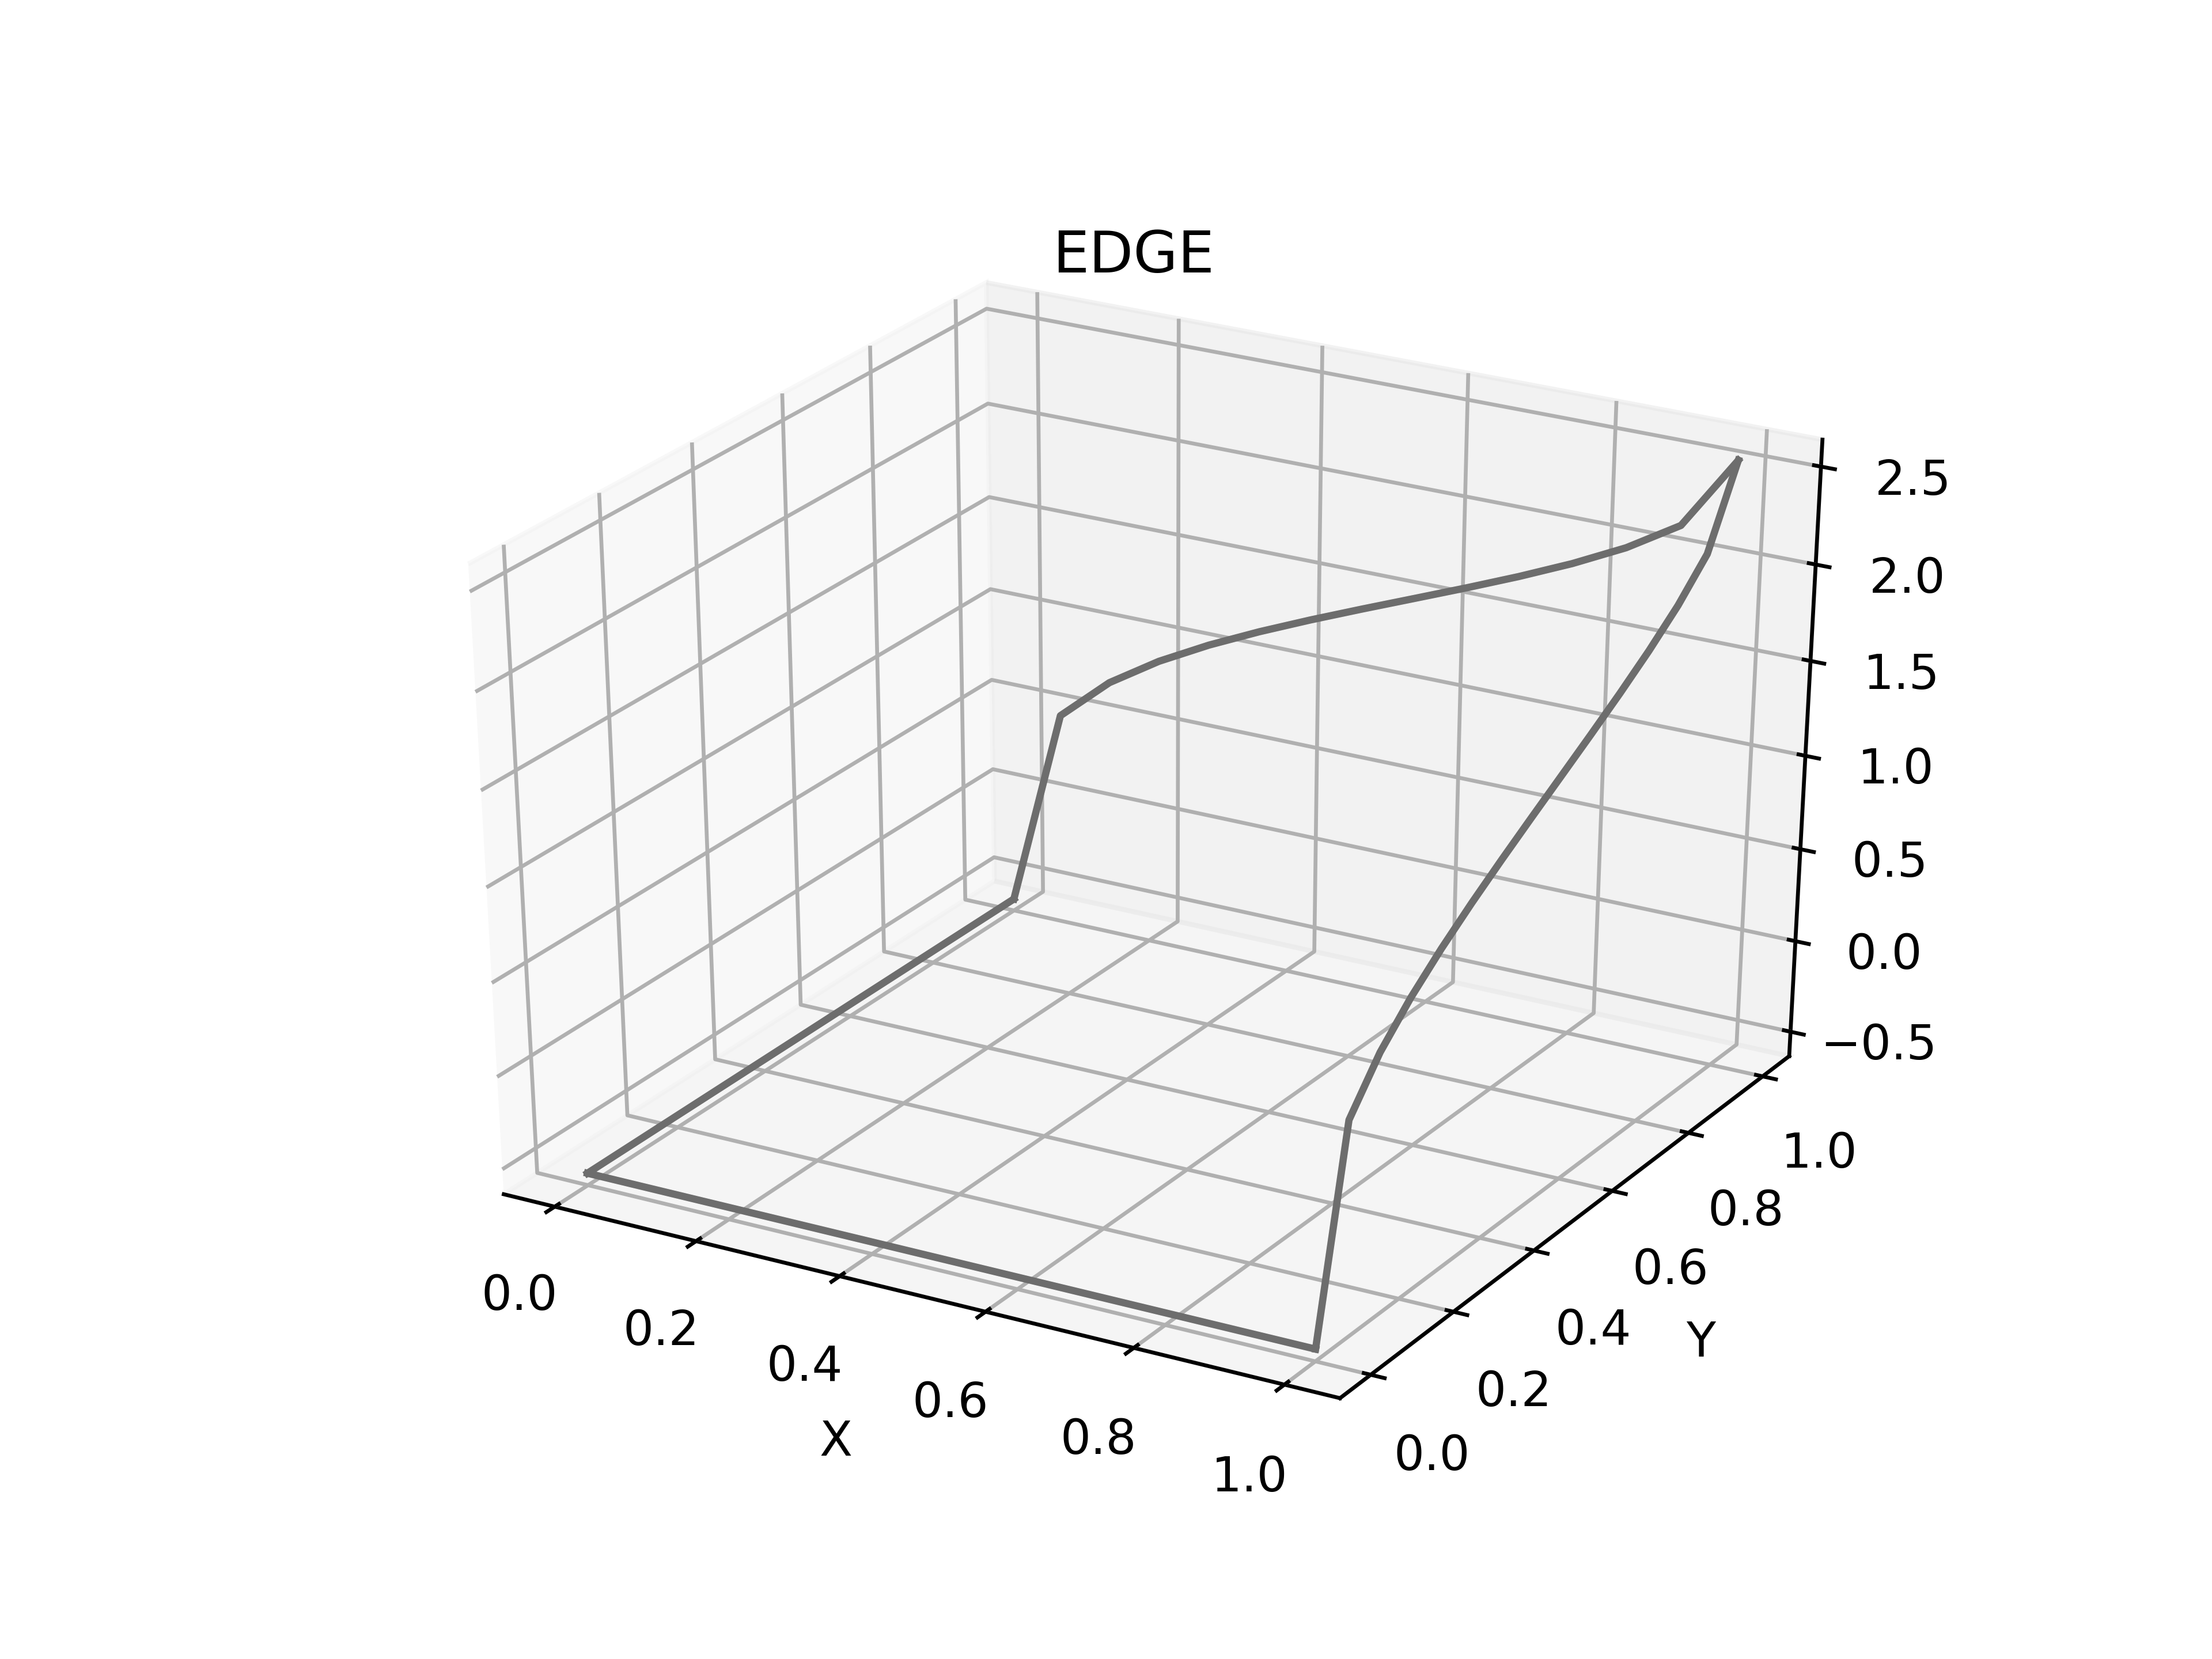
\includegraphics[width=0.3\columnwidth]{images/boundary_3.png}
    }
    \subfigure[$ r_4(x, y)=(1+\exp (x y))^{-1}$]
    {
    \centering
    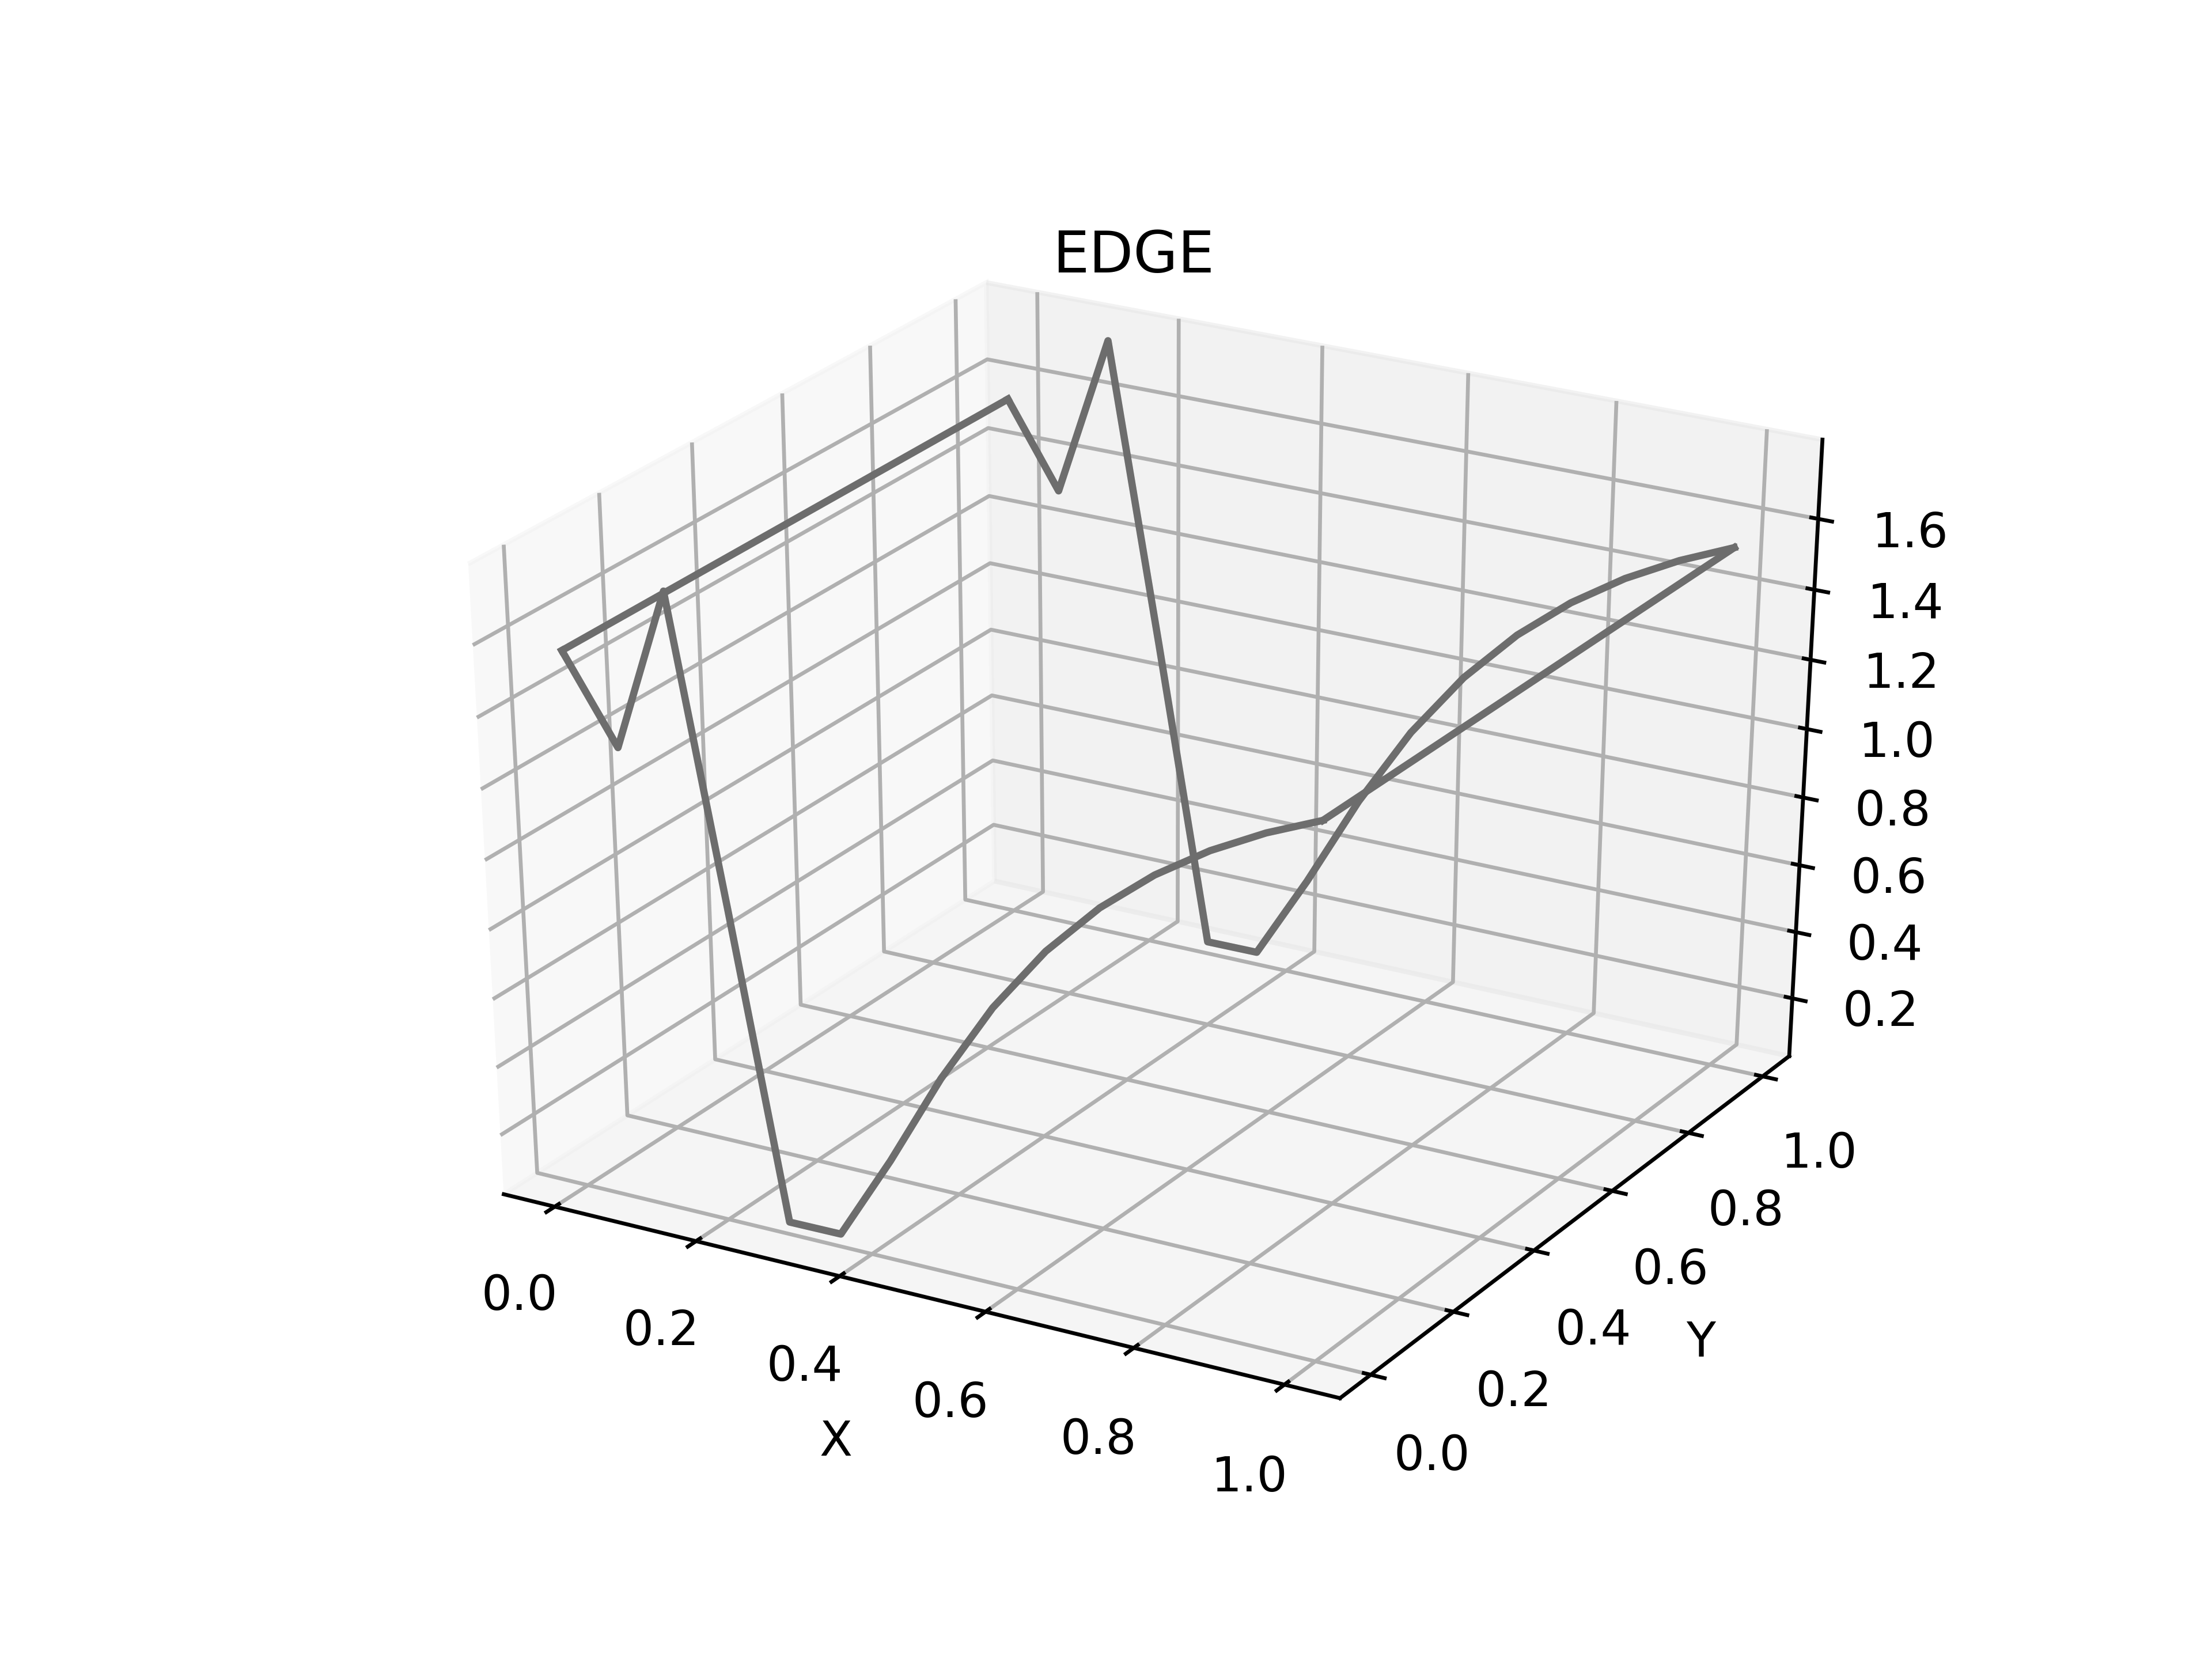
\includegraphics[width=0.3\columnwidth]{images/boundary_4.png}
    }
    \subfigure[$ r_5(x, y)=1+\arcsin (-1+2 \sqrt{x y})$]
    {
    \centering
    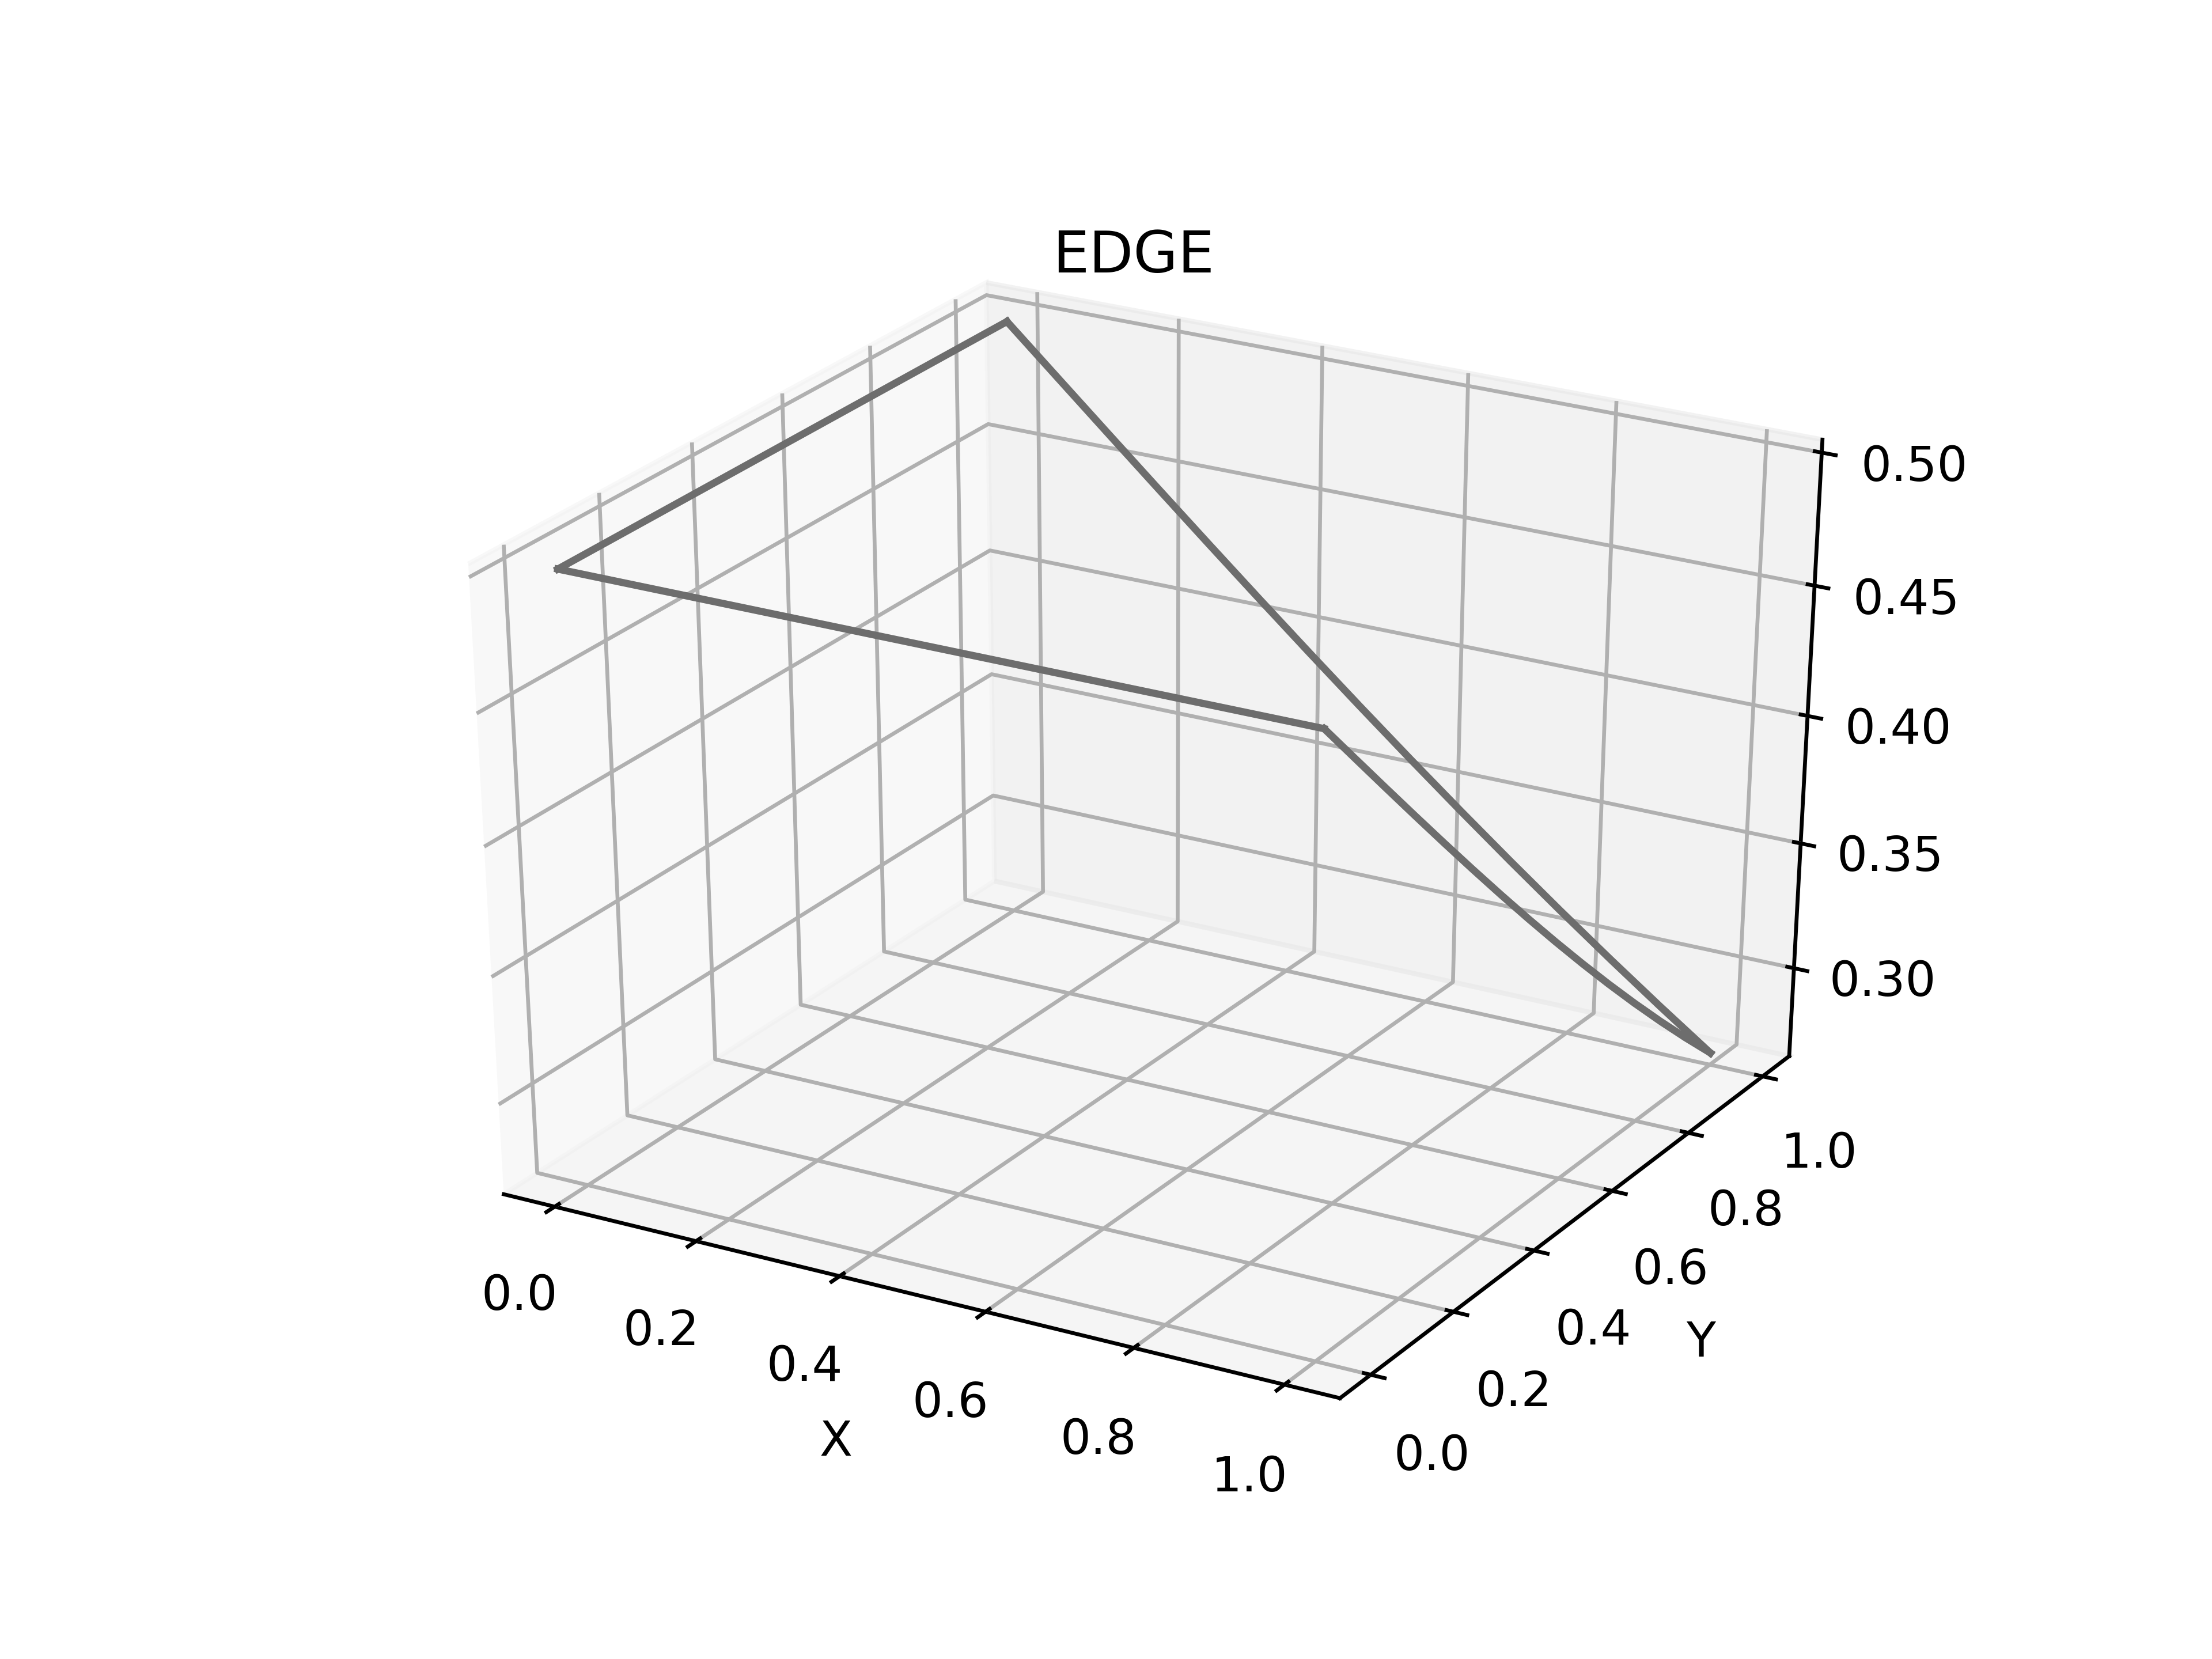
\includegraphics[width=0.3\columnwidth]{images/boundary_5.png}
    }
    \caption{Five Boundaries in the Minimal Surface Problem}
    \label{fig:boundary}  
\end{figure}
\subsubsection{Minimum Surface Results}
In order to demonstrate how the boundary function and discretization degree influence the minimal surface area, we choose globalized newton method to test these effects.
\subsubsection{Perfomance Analysis}
\subsubsection{Additional Techniques}
\subsection{Obstacle Problems}
As presented similarly in section 4.1, we firstly show different obstacles in the defiend boundary set via stochastic generation methods. We then choose projected gradient method to tackle the constrained optimization problem with different obstacle problems and illustrate corresponding minimum surface results. Lastly, We will equally present the perfomance camparing these two proposed algorithms. 
\subsubsection{Different Obstacles}
\subsubsection{Minimum Surface Results}
\subsubsection{Perfomance Analysis}



